\chapter{Data Governance and Management}
As we have said countless times up to this point, cloud computing is a very complex matter, the NIST definition can be found back in section 5.4 and the issues of the model are the following:
\begin{itemize}
    \item (Micro)Services composition
    \item Untrustworthy data
    \item High dynamics and flexibility
    \item Multi-domain evaluation
\end{itemize}
The natural evolution of cloud spanning an even bigger area is IoT, IoT is \textit{The intelligent connectivity of physical devices driving massive gains in efficency, business growth and quality of life}. \n
The first big step in that direction was made with 5G, high-speed connectivity with very low latency is one of the basic requirements to start setting up the needed infrastructure for a smart city. \n
In an IoT setting the cloud will have a layered and hierarchical structure with cloud data centers, that exchange informations with fog nodes that pre-process data coming from the edge of the cloud which are all the cameras and sensors embedded in smart systems. Having many sensors connected and collecting data every minute requires a very good metrics and analytics system to process the data coming from the edge and implement specific management functionalities. \n
It's obvious that the time has come to talk a bit about big data and more data driven techniques. \n
The 5 Vs of big data are the following:
\begin{itemize}
    \item Volume, the size of the data
    \item Velocity, the speed at which the data is generated
    \item Variety, the different types of data
    \item Veracity, The trustworthiness of the data in terms of accuracy
    \item Value, having data is of no use unless they can be turned into value
\end{itemize}
The data analytics pipeline is shown in figure 12
\begin{figure}
    \centering
    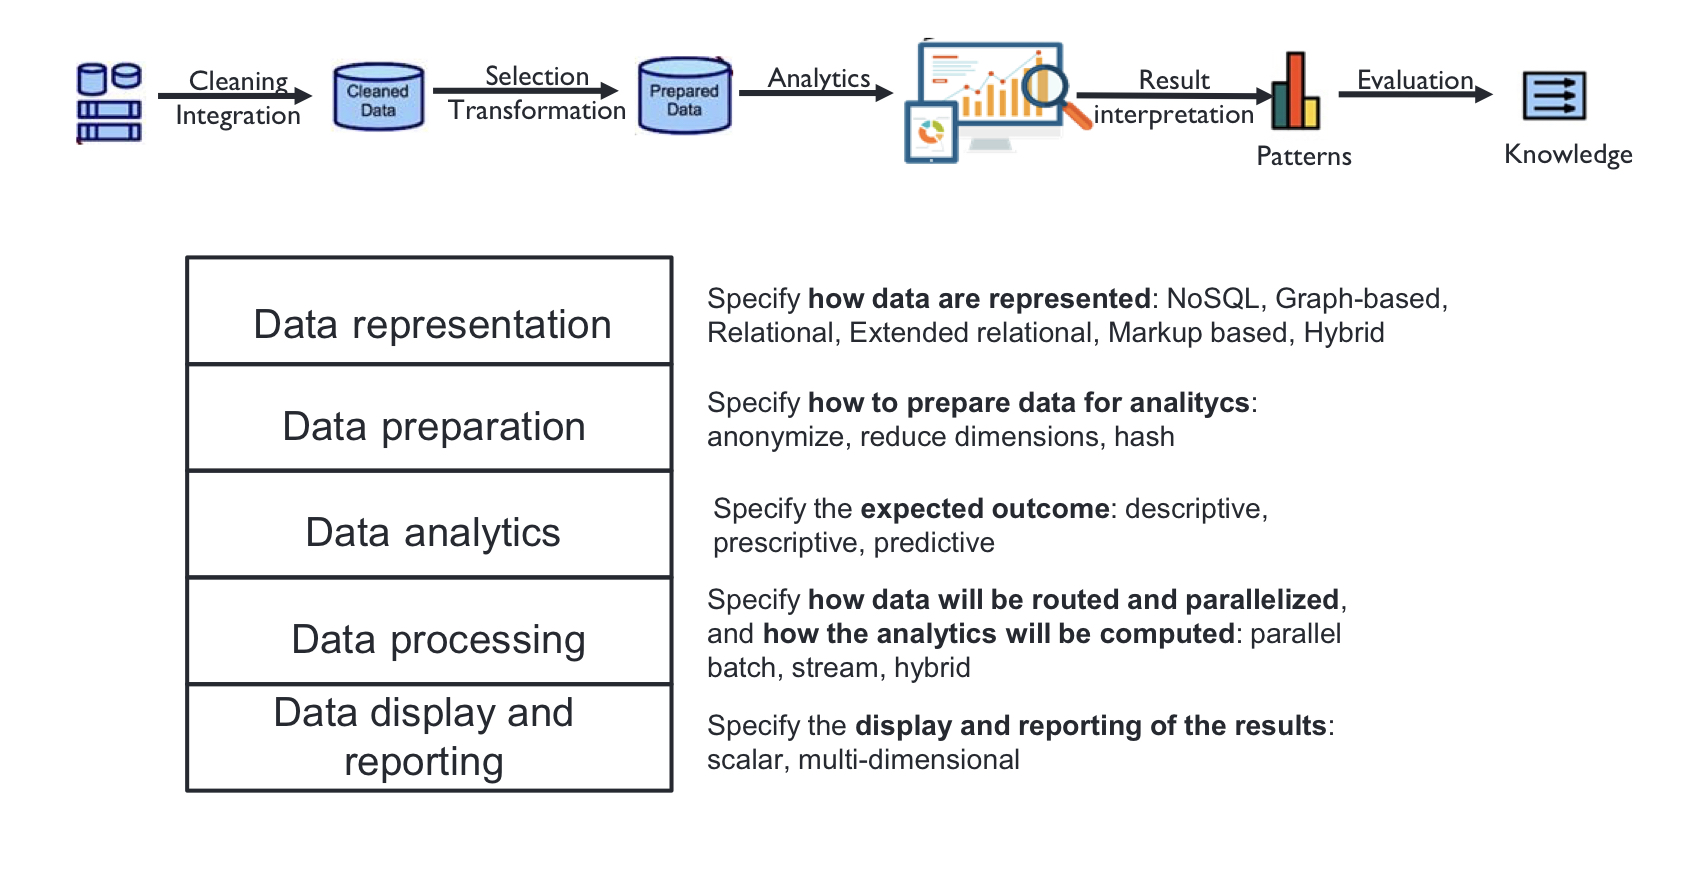
\includegraphics[scale=0.2]{Images/data_analytics_pipeline.jpeg}
    \caption{The data analytics pipeline}
\end{figure}
Since companies have seen how profitable can be a data-driven development process big data technologies have grown tremendousl in the past few years but there has been an incredible shortage of data scientists and data engineers, the demand is far from being met. \n
Only 30\% of businesses have a fully integrated data-analytics pipeline, 38\% of the businesses are struggling even with proofs of concept, key challenges associated with the development and management of Big Data initiatives are:
\begin{itemize}
    \item Lack of skills and clarity on Big Data technology (many people in the business do not even know that in data there is money to be made)
    \item Lack of general architecture and lack of standard processes
    \item Ineffective governance models
\end{itemize}
The biggest implementation challenges today in the field of Big Data are that: it's really hard to store and manage data in different places and formats, plus there is no coordintation in the field of big data / AI initiatives, solving the problem of handling massive amounts of data is not trivial both from an implementation and an engineering stand point, dated data and inability to operationalize insights and big data tool selection. \n
Getting into big data at this point in time can be done with many open source alternatives when it comes to both big data processing frameworks, storage and implementation languages. The incredible amount of alternatives allows companies to choose whichever technological stack they prefer without having to bind to one specific producer. \n
As I said, thanks to the power of alternatives, there are a bunch of commercial analytics platforms that are built on top of big data open source technologies (Apache Hadoop, Spark, Storm, etc...) the leaders in this space are Cloudera, Hortonworks and IBM insights, this is a summary of their features:
\begin{itemize}
    \item Provide enterprise-ready Hadoop distributions
    \item Management of Hadoop clusters
    \item Performance analytics
    \item Security and SLA monitoring
    \item Support for integrated marketing solutions
\end{itemize}
When it comes to data governance most technologies also offer data preparation functionalities like: ETL or ELT (Extract, Transform and Load). \n
Data storage and preparation tools offer:
\begin{itemize}
    \item Data inventory
    \item Metadata management
    \item Data quality
    \item Data integration
    \item Data security
    \item Fault tolerance
    \item ELT, ETL
    \item SLA monitoring
\end{itemize}
There are many providers when it comes to analytics and visualization technology. A summary of the offered features is:
\begin{itemize}
    \item Graphical interface to design analytics model
    \item Store the analysis result to different databases
    \item Provide data training and validation environment
\end{itemize}
Up to this moment we have basically reinforced the fact that there is a plethora of different big data technologies to choose from, picking a stack that suits the needs of the client can be a very complex task, it's important to keep in mind the fact that there is no single big data technology and balance between bottom-up and top-down approaches should be found. An example of the selection process is shown in figure 13.
\begin{figure}
    \centering
    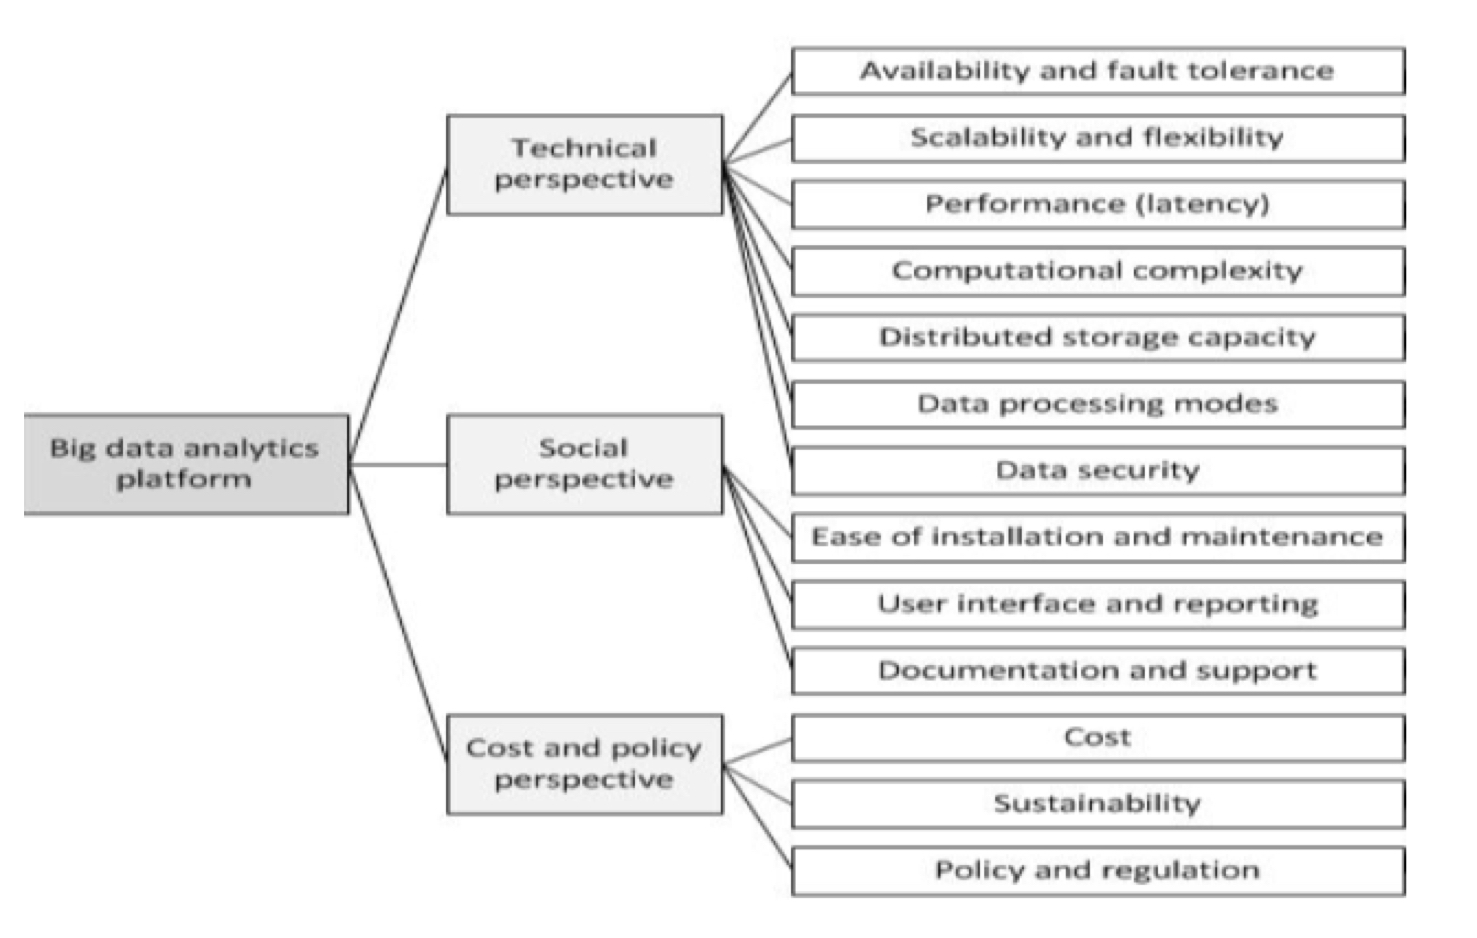
\includegraphics[scale=0.2]{Images/tech_selection_process.jpeg}
    \caption{Example of criterion to select big data technologies}
\end{figure}
\section{Big Data as a Service (BDaaS)}
We have said that entering the world of big data is a hustle, we have also said that there are not enough people to meet the work demand in the field and that there is a heck of a lot of money to be made from the good use of users data. \n
Point is? \n
A new company wanting to enter the scene (not necessarily in the tech world) and needing a big data system gets to a point where they find themselves in a situation where they have options, too many options, and no easy solution to all the mess. \n
Somebody thought it would be really cool to merge cloud business logic with big data. What if, I gave you a ready to use infrastructure, no further knowledge required, to handle your big data needs, in exchange for a fee? No need to lose your wits on a big data infrastructure implementation, that's for sure. \n
BSaaS are not just about storage and cost, these solutions offer built-in systems for artificial intelligence and analytics, you can accomplish some pretty impressive results without having to have a huge team of data analysts, scientists and architects around you. \n
The advantages of BDaaS are pretty obvious:
\begin{itemize}
    \item Makes managing big data easier
    \item Opens up big data for a range of medium-sized businesses
    \item It's a very low cost solution compared to the alternative of running your own metal (just like with the clud)
\end{itemize}
There are three different BDaaS models:
\begin{itemize}
    \item Big data infrastructure as a service, it's a IaaS offer including basic data services from a cloud serivce provider.
    \item Big data platform as a service, is a PaaS offer for an all-round big data stack.
    \item Big data software as a service, a SaaS offer which is self contained in a single tool.
\end{itemize}
How does the big data IaaS model work? There is a data layer, consisting of either: Hadoop, NoSequel databases and Relational databases; a compute layer, which can either be: Self-built ETL scripts, Commercial ETL tools or open source processing tools. \n
If we climb the stack a PaaS model can be (if we consider Amazon's implementation) a standard Hadoop implementation with:
\begin{itemize}
    \item Data ingestion, logs file data from any data source
    \item Amazon S3 data storage layer
    \item Analytics and visualization
\end{itemize}
A similar setup is implemented by competitors. \n
Last but not least, getting to the SaaS level, a fully hosted big data stack that includes everything from data storage to data visualization has the following:
\begin{itemize}
    \item Data layer
    \item Integration layer, pulls the data out of the database and into a flexible modeling layer
    \item Processing layer
    \item Analytics and BI layer
\end{itemize}
The differences between the various models can be summarized as follows:
\begin{itemize}
    \item IaaS is way more expensive than the other two models but allows almost complete control over resources and allows a custom implementation of complex data pipelines. It is not an easy thing to handle and is an hardcore alternative.
    \item PaaS is a much easier thing to master, it allows for a decent level of customization and control but it also requires a good level of expertise to handle compared to SaaS options.
    \item SaaS is a very low cost solution which is not that customizable but can tick many boxes for low to medium sized companies.
\end{itemize}
\section{Apache pipeline}
The Apache pipeline is shown in Figure 14 and includes the Hadoop framework, which is designed to store and process large amounts of data on clusters made of commodity hardware. It constitutes the lowest layer of the architecture and provides storage and resource management. \n
It also provides the Map Reduce processing model that allows concurrent scanning of multiple files, the model does not suffer from data intensive activities. \n
Hadoop is a distributed filesystem written in Java, based on the concept of distributing blocks across a series of different nodes. Hive is a structured data warehouse based on Hadoop capable of managing large datasets that reside in distributed storage.
\begin{figure}
    \centering
    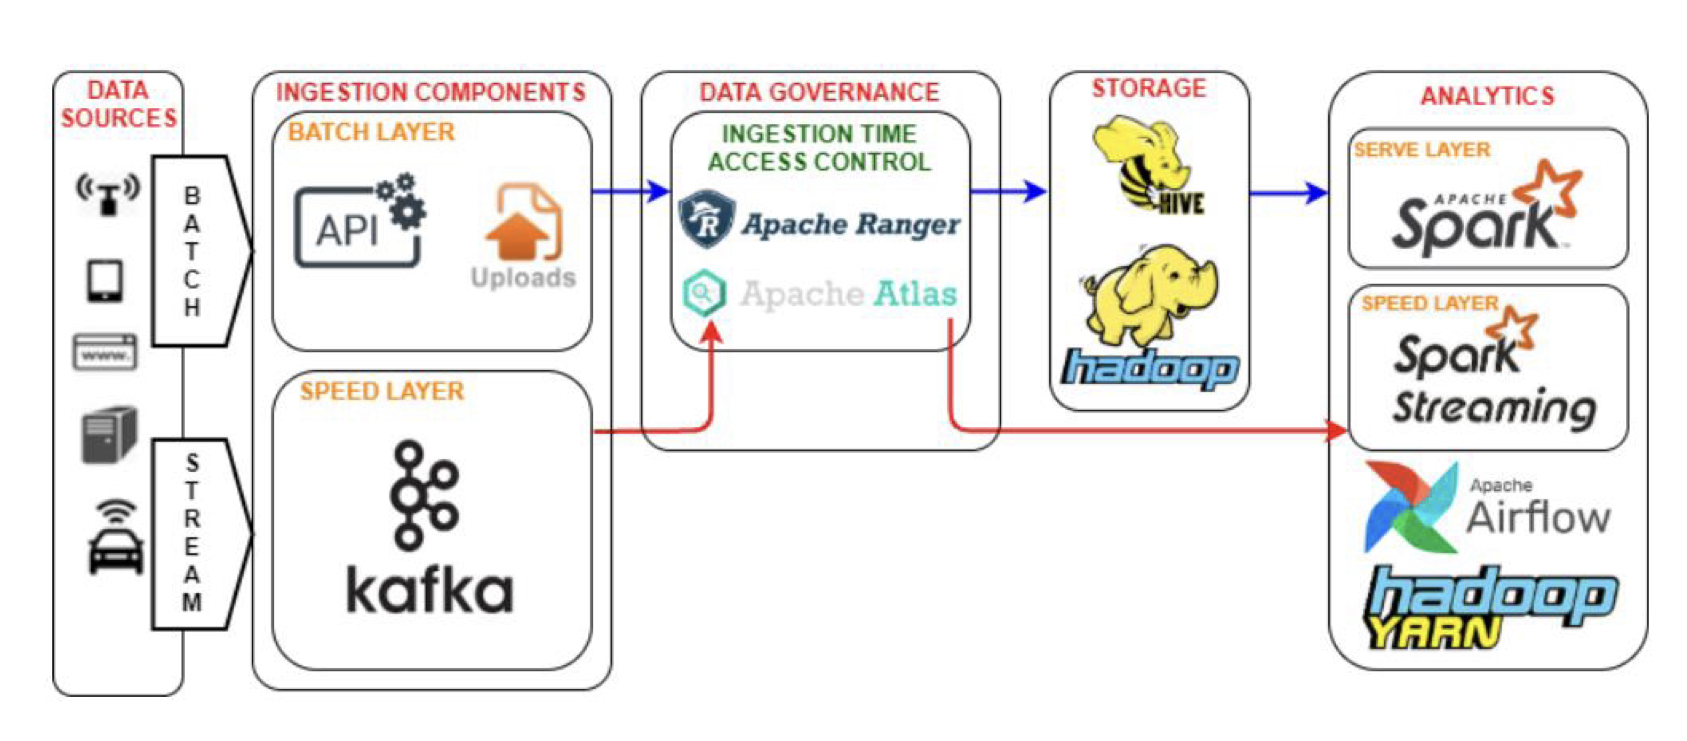
\includegraphics[scale=0.2]{Images/apache_architecture.jpeg}
    \caption{The Apache data pipeline}
\end{figure}
For the analytics section there is:
\begin{itemize}
    \item Hadoop YARN, which is the resource manager of the Hadoop cluster.
    \item Apache Spark, which is an analytics engine for large scale data processing, along with it there is Spark streaming that allows for large-scale stream (Kafka does stream ingestion) processing.
    \item Apache Airflow i an orchestrator of processing pipelines aimed at providing scheduling and monitoring capabilities.
\end{itemize}
Batch ingestion is handled via common APIs (like REST).
\section{Enterprise Data governance}
I think that I've skipped on the concept for a long while, what is Data Governance?
According to wikipedia: \textit{data governance is a data management concept concerning the capability that enables an organization to ensure that high data quality exists throughout the complete lifecycle of the data, and data controls are implemented that support business objectives}. \n
In the world of enterprise the point is to provide a common approach to data governance across all systems and data within the organization. An enterprise data governance should be:
\begin{itemize}
    \item Transparent - governance standards and protocols must be clearly defined and available to all.
    \item Reproducible - recreate the relevant data landscape at a point in time should be possible.
    \item Aubditable - all relevant events and assets must be traceable with appropriate historical lineage.
    \item Consistent - compliance practices must be consistent.
\end{itemize}
If we get back to the example of the Apache sute, two components play fundamental role for data governance:
Ranger (which is a policy editor and handles access control) and Atlas (which handles fine-grained data control via tagging). \n
\subsection{Apache Ranger}
Ranger gives centralized authorization and auditing across Hadoop components, it has an extensible architecture with custom policy conditions, context enrichers and more. \n
Policies are rules that decide how and who can access specific sets of resources and resource classifications. There are different policy types:
\begin{itemize}
    \item Access authorization based on resources or resource classification
    \item Row filter, column-masking based on policies, that can be done by restricting the rows accessible in a table based on users/groups/runtime-context or by masking/anonimizing sensitive columns.
\end{itemize}
\begin{figure}
    \centering
    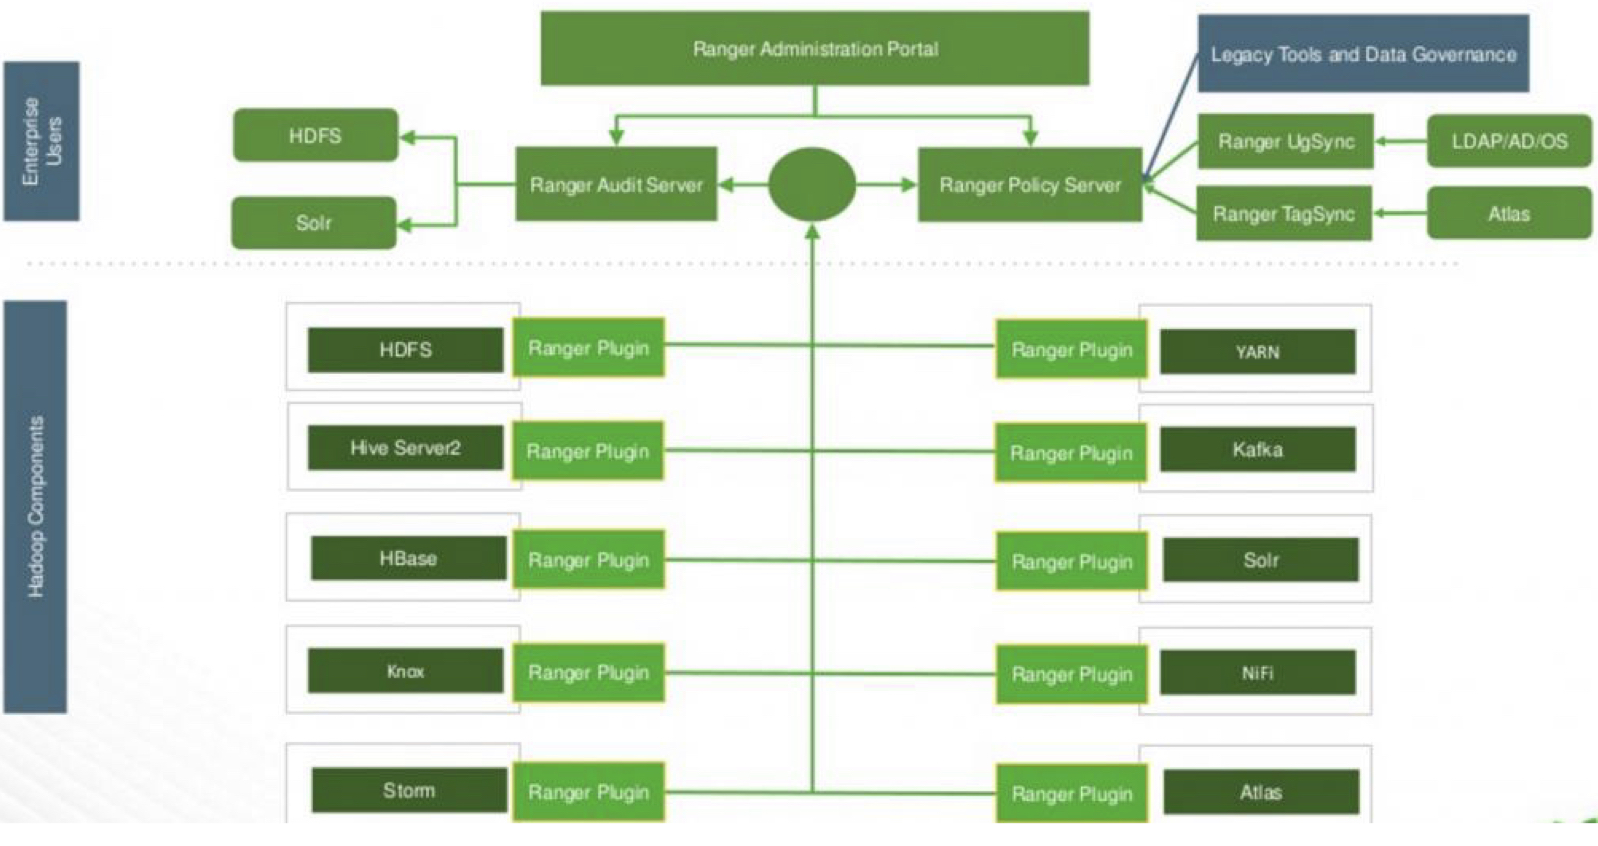
\includegraphics[scale=0.2]{Images/Ranger_architecture.jpeg}
    \caption{Ranger architecture}
\end{figure}
Ranger's architecture is shown in Figure 15. \n
The tags used in Ranger are created in Atlas and can be attatched to metadata, which can be a column, a table, an HDFS path, etc\dots \n
Plugin of each service saves tags info into policy and can be cached locally for fast retrieval. The flow of evaluation for tag policies is shown in Fiugre 16.
\begin{figure}
    \centering
    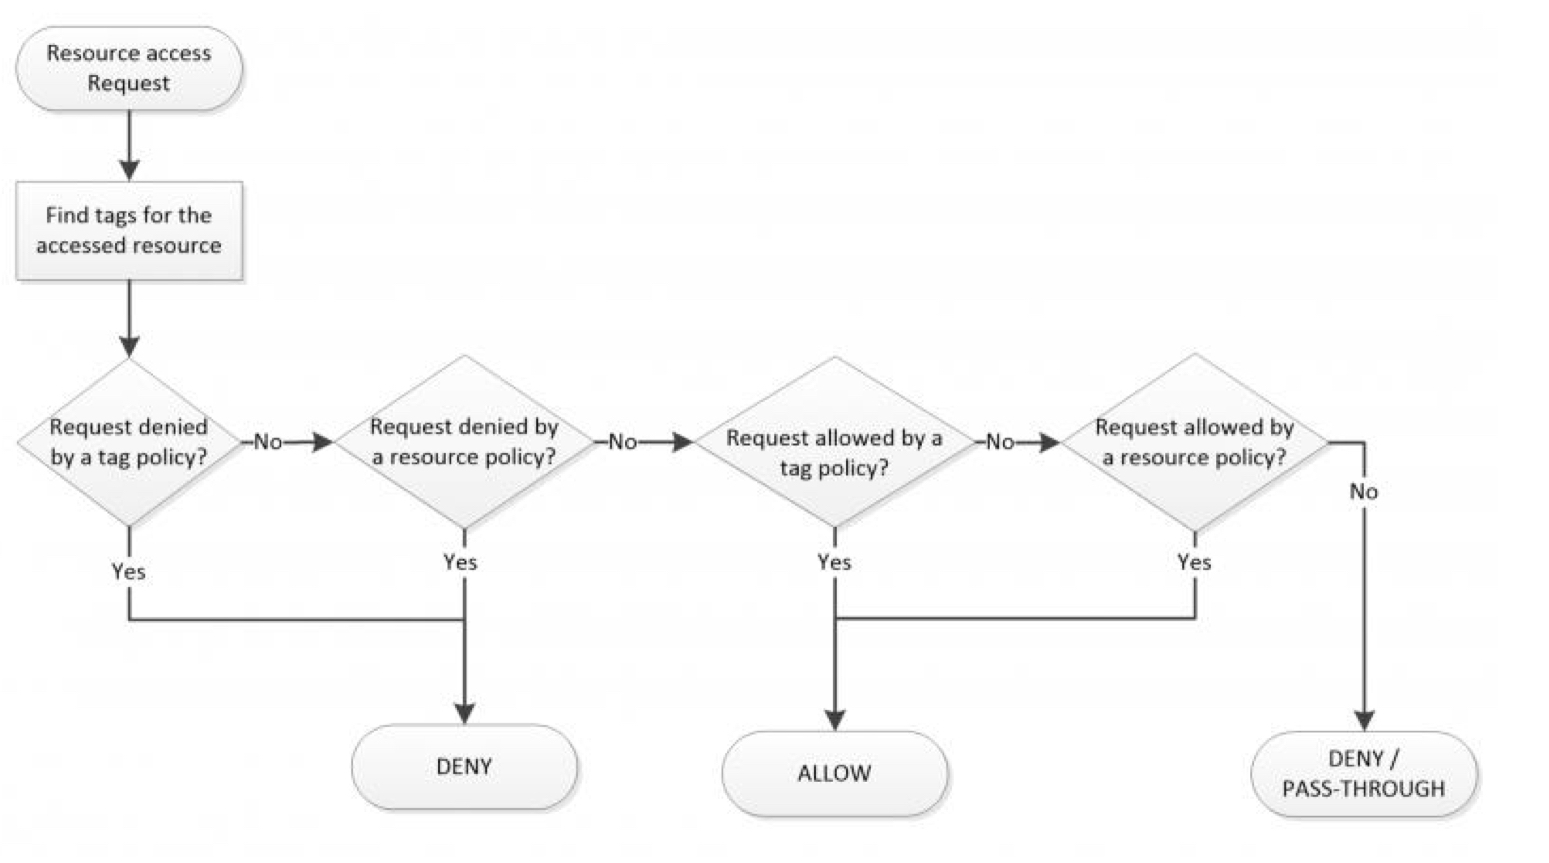
\includegraphics[scale=0.2]{Images/policies_evaluation.jpeg}
    \caption{The policies evaluation pipeline}
\end{figure}
\subsection{Apache Atlas}
Atlas provides open metadata management and governance capabilities for organizations to build a catalog of their data assets, classify and govern these assets and provide collaboration capabilities around these data assets for data scientists, analysts and the data governance team. \n
Atlas also provides:
\begin{itemize}
    \item Lineage
    \item Search/Discovery
    \item Support for Apache Ranger Security and Data Masking
\end{itemize}
Atlas keeps in memory a metadata repository with a flexible type system to capture schema/metadata of multiple components. \n
Is, obviously, perfectly integrated with Apache Hive, Storm, Falcon, Sqoop for metadata and lineage and also with Ranger for classification-based security. \n
It also provides APIs to support for more components. \n
\section{Data ingestion procedure}
\etl and \elt are two different ways of doing data ingestion and manipulation, the basic difference is that they are doing the same operations in a different fashion. \n
The basic operations are the following:
\begin{itemize}
    \item Extract - extraction refers to pulling the source data from the original database or data source. \etl puts data into a temporary staging area, while \elt sends data immediately into a data lake storage system.
    \item Transform - Transformation refers to the process of changing the structure of information, so it integrates with the target data system and the rest of the data in that system.
    \item Loading refers to the process of depositing the information into a data storage system.
\end{itemize}
\subsection{\etl}
\etl is typically used in data warehouses, the advantages of \etl are:
\begin{itemize}
    \item Pre structured nature of the OLAP (OnLine Analytical Processing) data warehouse
    \item Compliance to various laws like GDPR, HIPAA or CPAA.
    \item \etl was born over two decades ago and has been used a lot.
\end{itemize}
\subsection{\elt}
The \elt process also works with data lakes, a data lake is a special kind of data store accepting any kind of structured or unstructured data, there is no need to transform data before loading it. \n
The difference between \etl and \elt is that with \elt is possible to ingest anything and everything as data becomes accessible, \elt paired with a data lake lets you ingest and ever-expanding pool of raw data immediately as it becomes available. Plus it transforms only the data you need. \n
\elt is less reliable than \etl because \elt is still evolving. \n
To sum this up, the advantages of \elt are the following:
\begin{itemize}
    \item Flexibility and ease of storing new unstructured data.
    \item No need to develop complex \etl processes before data ingests.
    \item Saves developers and BI analysts time when dealing with new information.
    \item High speed.
    \item Low mantainance.
    \item Quicker loading.
\end{itemize}
\smallSpace
A lot of research still has to be done in the field, in particular:
\begin{itemize}
    \item Where and how to annotate data
    \item Where to do access control
    \item How to change AC to fir Big Data?
\end{itemize}